%!TEX TS-program = xelatex
%!TEX encoding = UTF-8 Unicode

% Project note
% 	1. 一定要用 xelatex 進行編譯,因為有牽扯到中文字
% 	2. 中文字體字體目前是使用Mac內建的中文字體
% 	3. Empty codeblocks will cause formatting problem

%%%%%% Page setting %%%%%%

%\documentclass[10pt,twocolumn,oneside]{article} %垂直兩欄、單面列印
%\setlength{\columnsep}{14pt} %兩欄模式的間距
%\setlength{\columnseprule}{0pt} %兩欄模式間格線粗細

\documentclass[10pt,oneside]{article}
\usepackage{pdflscape} % landscape mode
\usepackage{multicol} % two column
\usepackage{tocloft} 
\renewcommand\cftsecafterpnum{\vspace{-0.6ex}}
\renewcommand\cftsubsecafterpnum{\vspace{-0.6ex}}

\linespread{1} % 行距

\usepackage{enumitem} % Disable spacing in enumeration list
\setlist{nolistsep}

\usepackage{geometry} %定義邊界
\geometry{a4paper, total={170mm,257mm}, left=10mm, top=20mm, right=10mm}

%%%%%% Include special packages %%%%%%

%導入pdf文檔, \includepdf[pages={3,4}]{problem_statement.pdf}
\usepackage{pdfpages} 

%使用超連結, \href{http://codeforces.com/blog/entry/17974}{Codeforces}
\usepackage[colorlinks=true, urlcolor=cyan]{hyperref} 

%設定頁首頁尾
\usepackage{fancyhdr}	

 % 大量註解用 , \begin{comment}  % 註解開始,  \end{comment}  % 註解結尾
\usepackage{verbatim} 

\usepackage{amsmath}
\usepackage{array}

\usepackage{graphicx}
\graphicspath{ {images/} }

%%%%%% Font setting %%%%%%

\usepackage{fontspec} %加這個就可以設定字體 

\usepackage{xeCJK} %讓中英文字體分開設置
\setmainfont{Arial}
\setCJKmainfont{STKaiti} %設定中文為系統上的字型,而英文不去更動,使用原TeX字型
%\setmonofont{Courier} %等寬字體
\setmonofont{Oxygen Mono}

\XeTeXlinebreaklocale "zh" %這兩行一定要加,中文才能自動換行
\XeTeXlinebreakskip = 0pt plus 1pt 

%%%%%% lstsetting code setting %%%%%%

\usepackage{listings}
\usepackage{xcolor}

\definecolor{mygreen}{rgb}{0,0.6,0}
\definecolor{mygray}{rgb}{0.5,0.5,0.5}
\definecolor{mymauve}{rgb}{0.58,0,0.82}

\lstset{ %
  backgroundcolor=\color{black!5}, % set backgroundcolor,  choose the background color; you must add \usepackage{color} or \usepackage{xcolor}
  basicstyle=\footnotesize,   % the size of the fonts that are used for the code
  breakatwhitespace=false,   % sets if automatic breaks should only happen at whitespace
  breaklines=true,  % sets automatic line breaking
  captionpos=b,  % sets the caption-position to bottom
  frame=L, % add double line frame at the LHS of the code
  escapeinside={\%*}{*)},  % if you want to add LaTeX within your code
  keepspaces=true,  % keeps spaces in text, useful for keeping indentation of code (possibly needs columns=flexible)
  columns=flexible,
  commentstyle=\color{mygreen}, % comment style
  keywordstyle=\color{blue},  % keyword style
  %otherkeywords={*,...}, % if you want to add more keywords to the set  
  numbers=left, % where to put the line-numbers; possible values are (none, left, right)
  numbersep=7pt, % how far the line-numbers are from the code
  numberstyle=\tiny\color{mygray}, % the style that is used for the line-numbers
  stepnumber=1,  % the step between two line-numbers. If it's 1, each line will be numbered
  rulecolor=\color{black}, % if not set, the frame-color may be changed on line-breaks within not-black text (e.g. comments (green here))
  showspaces=false, % show spaces everywhere adding particular underscores; it overrides 'showstringspaces'
  showstringspaces=false, % underline spaces within strings only
  showtabs=false, % show tabs within strings adding particular underscores
  stringstyle=\color{mymauve},     % string literal style
  tabsize=4, % sets default tabsize to 4 spaces
  basicstyle=\footnotesize\ttfamily, %等寬字體 字體大小
  xleftmargin=\parindent,
  %title=\lstname % show the filename of files included with \lstinputlisting; also try caption instead of title
}

\lstdefinestyle{customc}{
  belowcaptionskip=1\baselineskip,
  breaklines=true,
  language=C++,
  showstringspaces=false,
  keywordstyle=\bfseries\color{green!40!black},
  commentstyle=\itshape\color{purple!40!black},
  identifierstyle=\color{blue},
  stringstyle=\color{orange},
}

\lstset{style=customc}



% sudo easy_install Pygments
% Add -shell-escape to compile flag
\usepackage{minted}

% Run in terminal for checking available styles: pygmentize -L styles
\usemintedstyle{friendly}
\definecolor{bg}{rgb}{0.95,0.95,0.95}
\newmintedfile[cppCode]{cpp}{ % [alias][code type]
%bgcolor=bg,
fontfamily=tt,
linenos=true,
numberblanklines=true,
numbersep=12pt,
numbersep=5pt,
gobble=0,
frame=leftline,
framerule=0.4pt,
framesep=2mm,
funcnamehighlighting=true,
tabsize=4,
obeytabs=false,
mathescape=false
samepage=false, %with this setting you can force the list to appear on the same page
showspaces=false,
showtabs =false,
texcl=false,
fontsize=\footnotesize,
breaklines=true,
}


%%%%%% 文件正式開始 %%%%%%

\begin{document} 

\begin{landscape} % landscape mode
\begin{multicols}{2} % two columns

%%%%%%%%%%%%%%%%%頁首%%%%%%%%%%%%%%%%%%%%

% for all other pages
\pagestyle{fancy}
% generate header
\fancyhead[L]{National Chung Cheng University -- CCU\_ToInfinityAndBeyond}
\fancyhead[R]{\thepage}
% \rhead{
\includegraphics[width=1cm]{buzz}}
% generate footer
%\fancyfoot[L]{\includegraphics[width=20pt]{pic.jpg}} %team profile picture
\fancyfoot[C]{for 2017 桂冠賽 (Built on: \today)}
\fancyfoot[R]{\thepage}

% for page 1
\fancypagestyle{plain}
{
% generate header
\fancyhead[L]{National Chung Cheng University -- CCU\_ToInfinityAndBeyond}
\fancyhead[R]{\thepage}
% generate footer
%\fancyfoot[L]{\includegraphics[width=20pt]{pic.jpg}} %team profile picture
\fancyfoot[C]{for 2017 桂冠賽 (Built on: \today)}
\fancyfoot[R]{\thepage}
}

% generate table of content on in a new page
\scriptsize
%\tableofcontents
\pagestyle{fancy}

%\newpage
\vfill
%\columnbreak

%%%%%%%%%%%%%%%%%正文%%%%%%%%%%%%%%%%%%%

%%%%%%%%%%%%%%%%機器設定%%%%%%%%%%%%%%%%%%

\begin{center}
	
\includegraphics[width=10cm]{buzz1}
\end{center}

\section{Contest Setup}

% \subsection{vimrc}
% \lstinputlisting[style=,basicstyle=\footnotesize\ttfamily]{contest_setup/vimrc}

% \subsection{bashrc}
% \lstinputlisting[style=,language=bash,basicstyle=\footnotesize\ttfamily]{contest_setup/bashrc}

% \subsection{Grep Error and Warnings}

% \begin{lstlisting}
% g++ main.cpp 2>&1 | grep -E 'warning|error'
% \end{lstlisting}

% \subsection{C++ template}
% \cppCode{contest_setup/main.cpp}

\subsection{Java template}
%\lstinputlisting{contest_setup/Main.java}
\inputminted{java}{contest_setup/Main.java}

\subsubsection{Java Issues}
{\normalsize
\begin{enumerate}
	\item Random Shuffle before sorting:\\ \mintinline{java}{Random rnd = new Random(); rnd.nextInt();}
	\item Use \mintinline{java}{StringBuilder} for large output
	\item Java has strict parsing rules. e.g. using \mintinline{java}{sc.nextInt()} to read a long will result in RE
	\item For class sorting, use code \mintinline{java}{implements Comparable<Class name>}. Or, use code \mintinline{java}{new Comparator<Interval>() {}} at \mintinline{java}{Collections.sort()} second argument
\end{enumerate}
}

\section{System Testing}

{\normalsize
\begin{enumerate}
	\item Setup vimrc and bashrc
	\item Test g++ and Java 8 compiler
	\item Look for compilation parameter and code it into bashrc
	\item Test if c++ and Java templates work properly on local and judge machine (bits, auto, and other c++11 stuff)
	\item Test "divide by 0" $\rightarrow$ RE/TLE?
	\item Make a complete graph and run Floyd warshall, to test time complexity upper bound
	\item Make a linear graph and use DFS to test stack size
	\item Test output with extra newline and spaces
	\item Go to $Eclipse \rightarrow preference \rightarrow Java \rightarrow Editor \rightarrow Content Assist$, add $.abcdefghijklmnopqrstuvwxyz$ to auto activation triggers for Java in Eclipse
\end{enumerate}
}

%%%%%%%%%%%%%%%%%忠告%%%%%%%%%%%%%%%%%%%%

\section{Reminder}

% 
\includegraphics{sorting3}

{\large
\begin{enumerate}
	\item 隊友的建議,要認真聽!要記得心平氣和的小聲討論喔!通常隊友的建議都會突破你盲點。
	\item 每一題都要小心讀,尤其是IO的格式和限制都要看清楚。%Read the problem statements carefully. Input and output specifications and constraints are crucial!
	\item 小心估計\textbf{時間複雜度} 和 \textbf{空間複雜度}%Estimate the \textbf{time complexity} and \textbf{memory complexity} carefully.
	\item Coding 要兩人一組,要相信你的隊友的實力!
	\item 1WA 罰 20 分鐘! \textbf{放輕鬆,不要急},多產幾組測資後再丟。%Time penalty is 20 minutes per WA, \textbf{don't rush}!
	\item 範測一定要過!產個幾組極端測資,例如 input 下限、特殊 cases 0, 1, -1、空集合等等 %Sample test cases must all be tested and passed before every submission! Test the corner cases, such as 0, 1, -1. Test all edge cases of the input specification.
	\item 比賽是連續測資,一定要全部讀完再開始 solve 喔!%For continuous input problems, be sure to read in all input BEFORE terminating and start processing next the input.
	\item Bus error: 有\mintinline{c++}{scanf, fgets} 但是卻沒東西可以讀取了!可能有early termination但是時機不對。 % Bus error: the code has $scanf, fgets$ but have nothing to read! Check if you have early termination but didn't handle it properly.
	\item 圖論一定要記得檢查連通性。最簡單的做法就是loop過所有的點%Check connectivity of the graph if the problem statement doesn't say anything (just loop over all nodes!)
	\item \mintinline{c++}{long long = int * int} 會完蛋%$long\ long = int * int$ won't work!
	\item \mintinline{c++}{long long int} 的位元運算要記得用 \mintinline{c++}{1LL << 35} %Shifting for $long long int$ should be something like $1LL << 35$
	%\item Don't use anonymous struct
	\item 記得清理Global variable
	\item 建圖時要注意有無重邊!
\end{enumerate}
}

\section{Topic list}

{\large
\begin{enumerate}
	\item 列舉、窮舉 enumeration
	\item 貪心 greedy 
	\item 排序 sorting, topological sort
	\item 二分搜 binary search (數學算式移項合併後查詢)
	\item 爬行法 (右跑左追)Two Pointer
	\item 離散化
	\item Dynamic programming, 矩陣快速冪
	\item 鴿籠原理 Pigeonhole 
	\item 最近共同祖先 LCA (倍增法, LCA轉RMQ)
	\item 折半完全列舉 (能用vector就用vector)
	\item 離線查詢 Offline (DFS, LCA)
	\item 圖的連通性 Directed graph connectivity -> DFS. Undirected graph -> Union Find
	\item 因式分解
	\item 從答案推回來
	\item 寫出數學式,有時就馬上出現答案了! % CF Div2 R372 C
	\item 奇偶性質
\end{enumerate}
}

%%%%%%%%%%%%%%%%實用代碼%%%%%%%%%%%%%%%%%%

\section{Useful code}

\subsection{Leap year $O(1)$}

\mintinline{c++}{(year % 400 == 0 || (year % 4 == 0 && year % 100 != 0))}

\subsection{Fast Exponentiation $O(log(exp))$}

{\normalsize Fermat's little theorem: 若 $m$ 是質數,則$a^{m-1} \equiv 1 \pmod m$}

\cppCode{useful_code/fast_pow.cpp}

\subsection{Mod Inverse $ O(log n) $}

{\normalsize 
Case 1: $gcd(a, m) = 1$:  ax + my = gcd(a, m) = 1 (use ext$\_$gcd) \\

\noindent Case 2: $m\ is\ prime$: $a^{m - 2} \equiv a^{-1} mod\ m$ 
}

\subsection{GCD $O(log( min(a + b) ))$}

{\large 注意負數的case! C++ 是看被除數決定正負號的。}

\begin{minted}{c++}
ll gcd(ll a, ll b)
{
    return b == 0 ? a : gcd(b, a % b);
}
\end{minted}

\subsection{Extended Euclidean Algorithm GCD $O(log( min(a + b) ))$}

{\normalsize 
Bezout identity $ax + by = gcd(a, b)$, where $\mid x \mid \leq \frac b d$ and $\mid y \mid \leq \frac a d$.
}

\cppCode{useful_code/ext_gcd.cpp}

\subsection{Prime Generator $ O(n loglogn) $}
\cppCode{useful_code/prime_gen.cpp}

\subsection{C++ Reference}

\cppCode{useful_code/cppReference2.cpp}

%\subsubsection{scanf/printf reference}

%\subsubsection{Map}
%\cppCode{useful_code/map_API.cpp}

%\subsubsection{Set}
%\cppCode{useful_code/set_API.cpp}

%\subsubsection{Algorithm}
%\cppCode{useful_code/algorithm_API.cpp}

%\subsubsection{String}

%%%%%%%%%%%%%%%%%搜尋%%%%%%%%%%%%%%%%%%%%

\section{Search}

\subsection{Ternary Search $O(nlogn)$}

\begin{minted}{c++}
double l = ..., r = ....; // input
for(int i  = 0; i < 100; i++) {
   double m1 = l + (r - l) / 3, m2 = r - (r - l) / 3;
   if (f (m1) < f (m2)) // f - convex function
      l = m1;
   else
      r = m2;
}
f(r) - maximum of function
\end{minted}

% \subsection{N Puzzle}
% \cppCode{Search/n-puzzle.cpp}


%%%%%%%%%%%%%%%%資料結構%%%%%%%%%%%%%%%%%%

\section{Basic data structure}

\subsection{1D BIT}

\begin{minted}{c++}
// BIT is 1-based
const int MAX_N = 20000; //這個記得改!
ll bit[MAX_N + 1];

ll sum(int i) {
    int s = 0;
    while (i > 0) {
        s += bit[i];
        i -= (i & -i);
    }
    return s;
}

void add(int i, ll x) {
    while (i <= MAX_N) {
        bit[i] += x;
        i += (i & -i);
    }
}
\end{minted}

\subsection{2D BIT}

\begin{minted}{c++}
// BIT is 1-based
const int MAX_N = 20000, MAX_M = 20000; //這個記得改!
ll bit[MAX_N + 1][MAX_M + 1];

ll sum(int a, int b) {
    ll s = 0;
    for (int i = a; i > 0; i -= (i & -i))
        for (int j = b; j > 0; j -= (j & -j))
            s += bit[i][j];
    return s;
}

void add(int a, int b, ll x) {
    // MAX_N, MAX_M 須適時調整!
    for (int i = a; i <= MAX_N; i += (i & -i))
        for (int j = b; j <= MAX_M; j += (j & -j))
            bit[i][j] += x;
}
\end{minted}

\subsection{Union Find}

\begin{minted}{c++}
const int MAX_N = 20000; // 記得改
struct UFDS {
    int par[MAX_N];

    void init(int n) {
        memset(par, -1, sizeof(int) * n);
    }

    int root(int x) {
        return par[x] < 0 ? x : par[x] = root(par[x]);
    }

    void merge(int x, int y) {
        x = root(x);
        y = root(y);

        if (x != y) {
            if (par[x] > par[y])
                swap(x, y);
            par[x] += par[y];
            par[y] = x;
        }
    }
};
\end{minted}

\subsection{Segment Tree}
\cppCode{DS/segmentTree2.cpp}

\subsection{Sparse Table}
\cppCode{DS/sparse_table.cpp}

%%%%%%%%%%%%%%%%%%樹%%%%%%%%%%%%%%%%%%%%

\section{Tree}

\subsection{LCA}
\cppCode{Tree/lca.cpp}

\subsection{Tree Center}
\cppCode{Tree/TreeCenter.cpp}

% \subsection{Treap}
% \cppCode{Tree/treap.cpp}

%%%%%%%%%%%%%%%%%圖論%%%%%%%%%%%%%%%%%%%

\section{Graph}

\subsection{Articulation point / Bridge}
\cppCode{graph/ArticulationPointAndBridge-1.cpp}

\subsection{2-SAT}

{\normalsize 
\begin{align*}
&p \lor (q \land r)  \\
&= ((p \land q) \lor (p \land r)) \\
&p \oplus q   \\
&= \lnot ( (p \land q) \lor (\lnot p \land \lnot q))     \\
&= (\lnot p \lor \lnot q) \land (p \lor q)    
\end{align*}
}

\begin{minted}{c++}
// 建圖
// (x1 or x2) and ... and (xi or xj)
// (xi or xj) 建邊
// ~xi -> xj
// ~xj -> xi

tarjan(); // scc 建立的順序是倒序的拓璞排序
for (int i = 0; i < 2 * N; i += 2) {
    if (belong[i] == belong[i ^ 1]) {
        // 無解
    }
}
for (int i = 0; i < 2 * N; i += 2) { // 迭代所有變數
    if (belong[i] < belong[i ^ 1]) { // i 的拓璞排序比 ~i 的拓璞排序大
        // i = T
    }
    else {
        // i = F
    }
}
\end{minted}

\subsection{CC}

\subsubsection{BCC}
{\normalsize 
%http://www.geeksforgeeks.org/biconnected-components/
以 Edge 做分界的話,stack 要裝入 (u - v), 並 pop 終止條件為 != (u - v) \\
以 Articulation point 做為分界 (code below),注意有無坑人的重邊 \\
注意,用SCC的code的話,只要多判一個 u 是否為 p, 如果是的話就直接 return (加在第21行之後)
}
%\cppCode{graph/BCC.cpp}

\subsubsection{SCC}

{\normalsize 
First of all we run DFS on the graph and sort the vertices in decreasing of their finishing time (we can use a stack).\\
Then, we start from the vertex with the greatest finishing time, and for each vertex v that is not yet in any SCC, do : for each u that v is reachable by u and u is not yet in any SCC, put it in the SCC of vertex v. The code is quite simple.
}

\cppCode{graph/SCC_AMO.cpp}

\subsection{Shortest Path}

{\normalsize 
Time complexity notations: V = vertex, E = edge \\
Minimax: $dp[u][v] = min(dp[u][v], max(dp[u][k], dp[k][v]))$ \\
}
%\subsubsection{Dijkatra}

%密集圖別用priority queue!\\
%http://amoshyc.github.io/ojsolution-build/template/graph/spfa.html
%\cppCode{graph/dijkatra.cpp}

\subsubsection{Dijkatra (next-to-shortest path) $O(VlogE)$}
{\normalsize 密集圖別用priority queue! }
% https://gist.github.com/amoshyc/f011abc6fad9b413c24b
\cppCode{graph/nextToShortestPath.cpp}

% \subsubsection{SPFA}
% \cppCode{graph/SPFA.cpp}

\subsubsection{Bellman-Ford $O(VE)$}
% UVa 558, 10449
\cppCode{graph/bellmanFord1.cpp}

\subsubsection{Floyd-Warshall $O(V^3)$}
{\normalsize 
The graph is stored using adjacency matrix. The initial state is $diagnal = 0$ and $others = INF$. (If $INF$ is int, use long long for the matrix)\\
If diagonal numbers are negative $\leftarrow$ cycle . \\
}

%UVA821 
\begin{minted}{c++}
for(int k = 0; k < N; k++)
    for(int i = 0; i < N; i++)
        for(int j = 0; j < N; j++)
            dp[i][j] = min(dp[i][j], dp[i][k] + dp[k][j]);
\end{minted}

\subsection{MST}

\subsubsection{Kruskal}

{\normalsize 
\begin{enumerate}
	\item Store the graph by $(weight, (from , to))$
	\item Sort the graph by $weight$ 
	\item Start from the smallest weight, and keep adding edges that won't form a cycle with the current MST set
	\item Early termination condition: $n - 1$ edges has been added, NOT size of the union-find set
\end{enumerate}
}

\subsubsection{Second MST}
% https://amoshyc.github.io/blog/template-ci-xiao-sheng-cheng-shu.html
\cppCode{graph/second_MST.cpp}

% \subsubsection{Prim}
% \cppCode{graph/prim.cpp}

\section{Flow}

\subsection{Max Flow (Dinic)}
%http://amoshyc.github.io/ojsolution-build/template/graph/max_flow.html
\cppCode{flow/dinic.cpp}

\subsection{Min Cost Flow}
%http://amoshyc.github.io/ojsolution-build/template/graph/min_cost_flow.html
\cppCode{flow/minCostFlow.cpp}

\subsection{Bipartite Matching, Unweighted}
%http://amoshyc.github.io/ojsolution-build/template/graph/bipartite_matching.html
\cppCode{flow/bipartiteMatching.cpp}

%%%%%%%%%%%%%%%%%字串%%%%%%%%%%%%%%%%%%%

\section{String}

\subsection{Rolling Hash}

{\normalsize 
\begin{enumerate}
	\item Use two rolling hashes if needed.  
	\item The prime for pre-calculation can be $137$ and $257$, for modulo can be $1e9 + 7$ and $0xdefaced$ 
\end{enumerate}
}

\cppCode{string/RollingHash.cpp}

\subsection{KMP}

\cppCode{string/KMP.cpp}

\subsection{Z Algorithm}

\cppCode{string/Z_Algorithm.cpp}

% \subsection{Trie}
% {\normalsize 
%http://amoshyc.github.io/ojsolution-build/template/ds/trie.html
% 注意count的擺放位置,視題意可以擺在迴圈外
% \cppCode{string/TrieAmoshyc.cpp}
% }

\section{Matrix}

\subsection{Gauss Jordan Elimination}
\cppCode{Matrix/gauss_jordan.cpp}

\subsection{Determinant}

{\normalsize 
整數版本
}

\cppCode{Matrix/matrix_det.cpp}

%%%%%%%%%%%%%%%%%幾何%%%%%%%%%%%%%%%%%%%

\section{Geometry}

{\normalsize 
\begin{enumerate}
	\item Keep things in integers as much as possible!
	\item Try not to divide
	\item If you have decimals, if they are fixed precision, you can usually just multiply all the input and use integers instead
\end{enumerate}
}

\subsection{EPS}

{\normalsize 
%$a > b \rightarrow a - b > 0 \rightarrow a - b > EPS$ (stands for positive)\\
%$a \geq b \rightarrow  a - b \geq 0 \rightarrow a - b > -EPS$ (stands for positive or zero)\\

$=0$: $fabs \leq eps$\\
$<0$: $ < -eps$\\
$>0$: $ > +eps$
}

%\subsection{Template}
% \cppCode{geometry/geometry_stanford.cpp}
\cppCode{geometry/my_geometry2.cpp}

\subsection{Rectangle area}
% https://amoshyc.github.io/blog/template-ju-xing-mian-ji-he.html
\cppCode{geometry/rect_area.cpp}

\section{Math}

\subsection{Euclid's formula (Pythagorean Triples)}

{\normalsize 
$a = p^2 - q^2 $\\
$b = 2pq \; \textbf{(always even)}$ \\
$c = p^2 + q^2$\\
}

\subsection{Difference between two consecutive numbers' square is odd}

{\normalsize 
$(k + 1)^2 - k^2 = 2k + 1$
}

\subsection{Summation}

{\normalsize 
$\sum_{k=1}^{n} 1= n$\\
$\sum_{k=1}^{n} k= \frac{n(n+1)}{2}$\\
$\sum_{k=1}^{n} k^2= \frac{n(n+1)(2n+1)}{6}$\\
$\sum_{k=1}^{n} k^3= \frac{n^2(n+1)^2}{4}$\\
}

% \subsection{FFT}
%http://amoshyc.github.io/ojsolution-build/template/math/fft.html
% \cppCode{Math/fft.cpp}

\subsection{Combination}

% Pi-You Uva 10943
\subsubsection{Pascal triangle}

\begin{minted}{c++}
#define N 210
ll C[N][N];

void Combination() {
    for(ll i=0; i<N; i++) {
        C[i][0] = 1;
        C[i][i] = 1;
    }

    for(ll i=2; i<N; i++) {
        for(ll j=1; j<=i; j++) {
            C[i][j] = (C[i-1][j] + C[i-1][j-1])%M; // if needed, mod it
        }
    }
}
\end{minted}

\subsubsection{Lucus}

\begin{equation}
\begin{split}&\binom{n}{m} \equiv \prod_{i=0}^k \binom{n_i}{m_i} \pmod p \\
\text{where}& \\
&n = n_kp^k+n_{k-1}p^{k-1}+\cdots +n_1p+n_0, \\
&m = m_kp^k+m_{k-1}p^{k-1}+\cdots +m_1p+m_0 \\
&p \text{ is prime}
c\end{split}
\end{equation}

\cppCode{Math/lucas.cpp}

\subsubsection{線性}

\begin{minted}{c++}
ll binomialCoeff(ll n, ll k)
{
    ll res = 1;
 
    if ( k > n - k ) // Since C(n, k) = C(n, n-k)
        k = n - k;
 
    for (int i = 0; i < k; ++i) // n...n-k / 1...k
    {
        res *= (n - i);
        res /= (i + 1);
    }
 
    return res;
}
\end{minted}

\subsection{Chinese remainder theorem}
%http://amoshyc.github.io/ojsolution-build/template/math/crt.html
\cppCode{Math/chineseRemainderTheorem.cpp}

\subsection{2-Circle relations}

{\normalsize 
$d$ = 圓心距, $R$, $r$ 為半徑 ($R \geq r$)\\
內切: $d = R - r$\\
外切: $d = R + r$\\
內離: $d < R - r$\\
外離: $d > R + r$\\
相交: $d < R + r$ 且 $d > R - r$
}

\subsection{Fun Facts}

{\normalsize 
\begin{enumerate}
	\item 如果 $\frac b a$ 是最簡分數,則 $1 - \frac b a$也是%http://amoshyc.github.io/ojsolution-build/cf/cf369/pe.html
\end{enumerate}
}

%%%%%%%%%%%%DP%%%%%%%%%%

\section{Dynamic Programming - Problems collection}
%\cppCode{DP/dp.cpp}
\VerbatimInput{DP/dp_noComment.txt}

%trig information
% 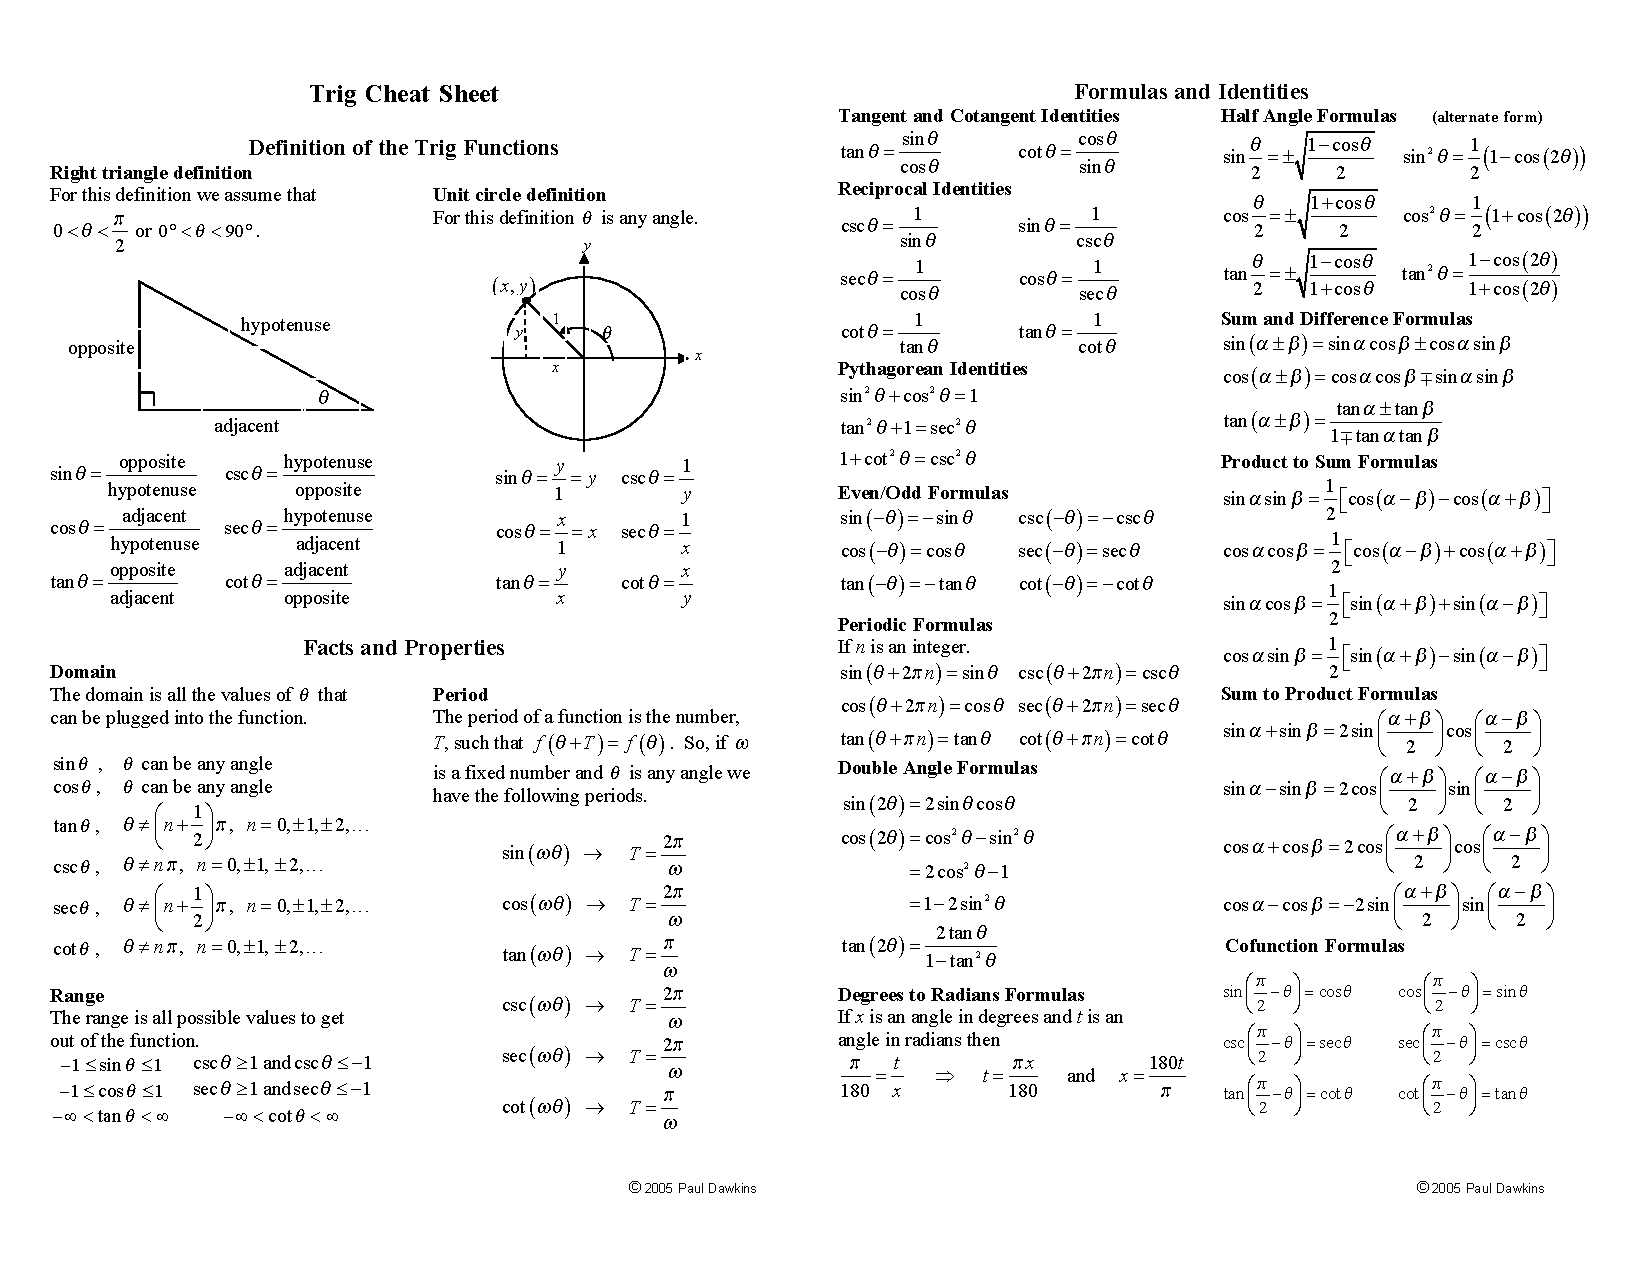
\includepdf[pages={1-},scale=1, angle=90]{Math/Trig_Cheat_Sheet_Reduced.pdf}

\end{multicols}
\end{landscape}

\end{document}
